\videotitle{Success Stories and Practical Recommendations}
%----------------------------------------------------------------------


\begin{frame}[c]{Large-scale meta-learning for hyperparameter optimization}

\begin{itemize}
    \item Facebook has an internal self-service machine learning system
    \item Non-ML departments can integrate highly optimized machine learning models into their workflow
    \item Hyperparameters of the ML models are optimized with Bayesian optimization
    \item Training data for the models changes over time \item Hyperparameters are constantly re-optimized using meta-learning Bayesian optimization as described in \lit{\href{https://arxiv.org/abs/1802.02219}{Feurer et al. 2018}}
    \begin{figure}
        \centering
        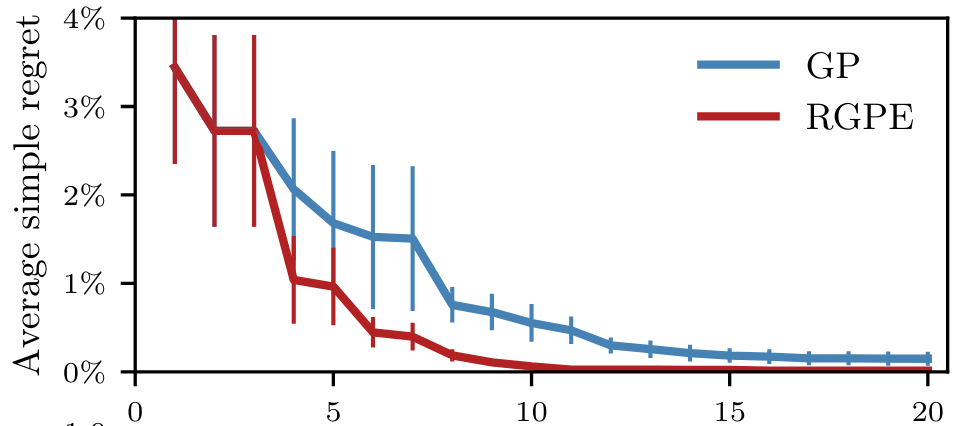
\includegraphics[width=0.5\textwidth]{../w07_hpo_speedup/images/success_stories/FB_RGPE.png}
        \caption{Bayesian optimization with meta-learning (RGPE) vs. vanilla Bayesian optimization (GP)}
    \end{figure}
\end{itemize}

\end{frame}

%-----------------------------------------------------------------------

\begin{frame}[c]{Auto-sklearn}
Extension of Auto-WEKA with focus on speed improvements and robustness:
\begin{figure}
    \centering
    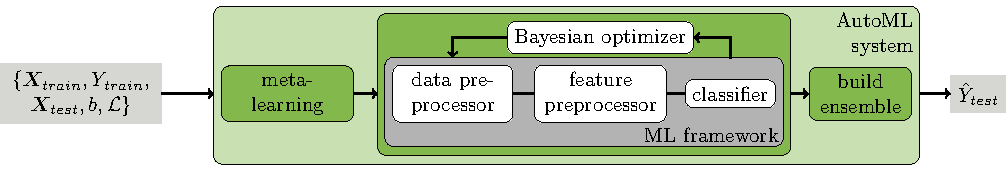
\includegraphics[width=0.9\textwidth]{images/success_stories/automlworkflow.pdf}
\end{figure}
\begin{itemize}
    \item Uses Meta-learning to warmstart Bayesian optimization
    \item Won the 1st AutoML challenge
    \item Open source (BSD) and trivial to use:
\end{itemize}
\begin{figure}
    \centering
    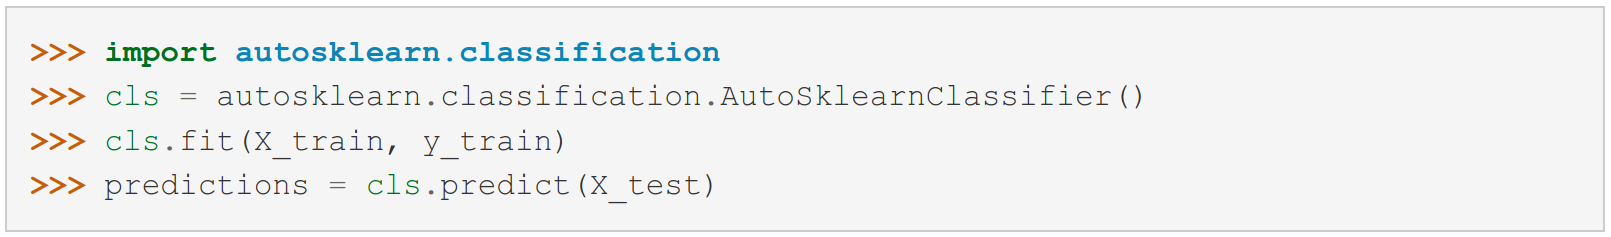
\includegraphics[width=0.85\textwidth]{images/success_stories/Auto-sklearn_01.png}
\end{figure}
Available at \url{https://automl.github.io/auto-sklearn}
\end{frame}

%-----------------------------------------------------------------------
\begin{frame}[c]{BOHB}

\myit{
	\item Robust and efficient 
	\item Only published in 2018, adopted by the community very quickly 
\begin{figure}
    \centering
    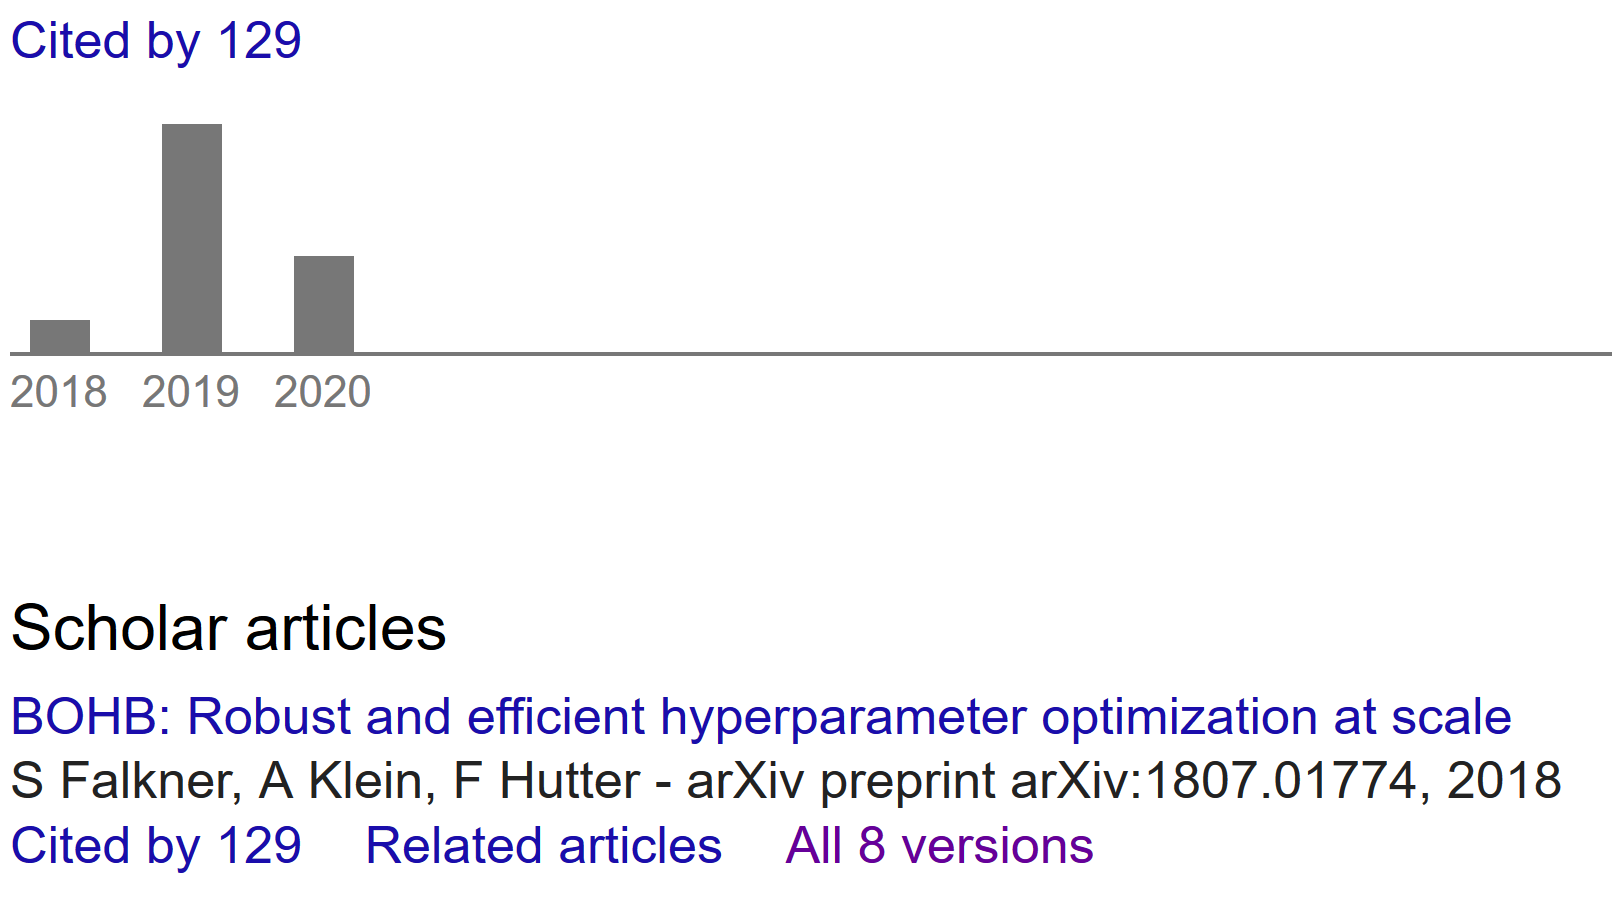
\includegraphics[height=4cm]{../w07_hpo_speedup/images/success_stories/BOHB-citations.png}
\end{figure}
\vspace*{0.4cm}
	\item Available at \url{https://github.com/automl/HpBandSter}
\begin{figure}
    
\includegraphics[height=0.6cm]{../w07_hpo_speedup/images/success_stories/BOHB-repo-stats.png}
\end{figure}
}

\end{frame}
%-----------------------------------------------------------------------

%-----------------------------------------------------------------------
\begin{frame}[c]{PoSH-Auto-sklearn} \lit{\href{https://ml.informatik.uni-freiburg.de/papers/18-AUTOML-AutoChallenge.pdf}{Feurer et al. 2018}}
Idea: integrate successive halving for further speed improvements:
\begin{itemize}
    \item Uses task-independent Meta-learning to warmstart Bayesian optimization
    \myit{
        \item Therefore, no need for (potentially unreliable) meta-features
    }
    \item Uses Successive Halving to quickly go through proposed configurations
    \myit{
        \item Therefore, scales better to larger datasets
    }
    \item Won the 2nd AutoML challenge
\end{itemize}

\begin{figure}
    \centering
    \includegraphics[width=\textwidth]{images/success_stories/automl_bo_po_es.png}
\end{figure}

\end{frame}

%-----------------------------------------------------------------------
\begin{frame}[c]{Auto-sklearn 2.0}

\begin{columns}

\column{0.4\textwidth}
\vskip 35pt
Idea: automatically choose:
\begin{itemize}
    \item holdout or cross-validation
    \item optimization on the full budget or optimization with successive halving
\end{itemize}
using algorithm selection
\vskip 10pt
Yields huge improvements over Auto-sklearn 1.0.

\column{0.6\textwidth}
\begin{figure}
    \centering
    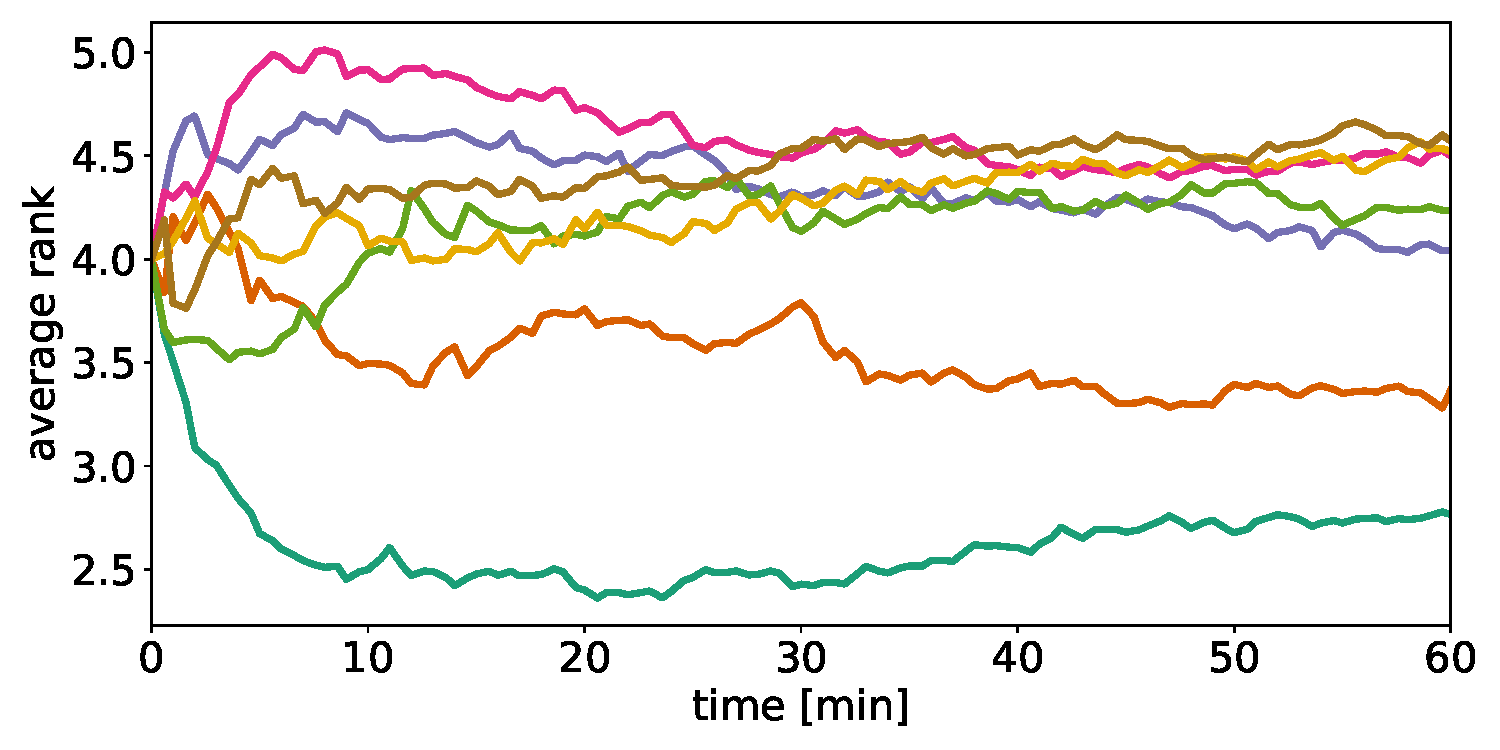
\includegraphics[width=\textwidth]{../w07_hpo_speedup/images/success_stories/RQ1_60MIN_ens_rank.pdf}
    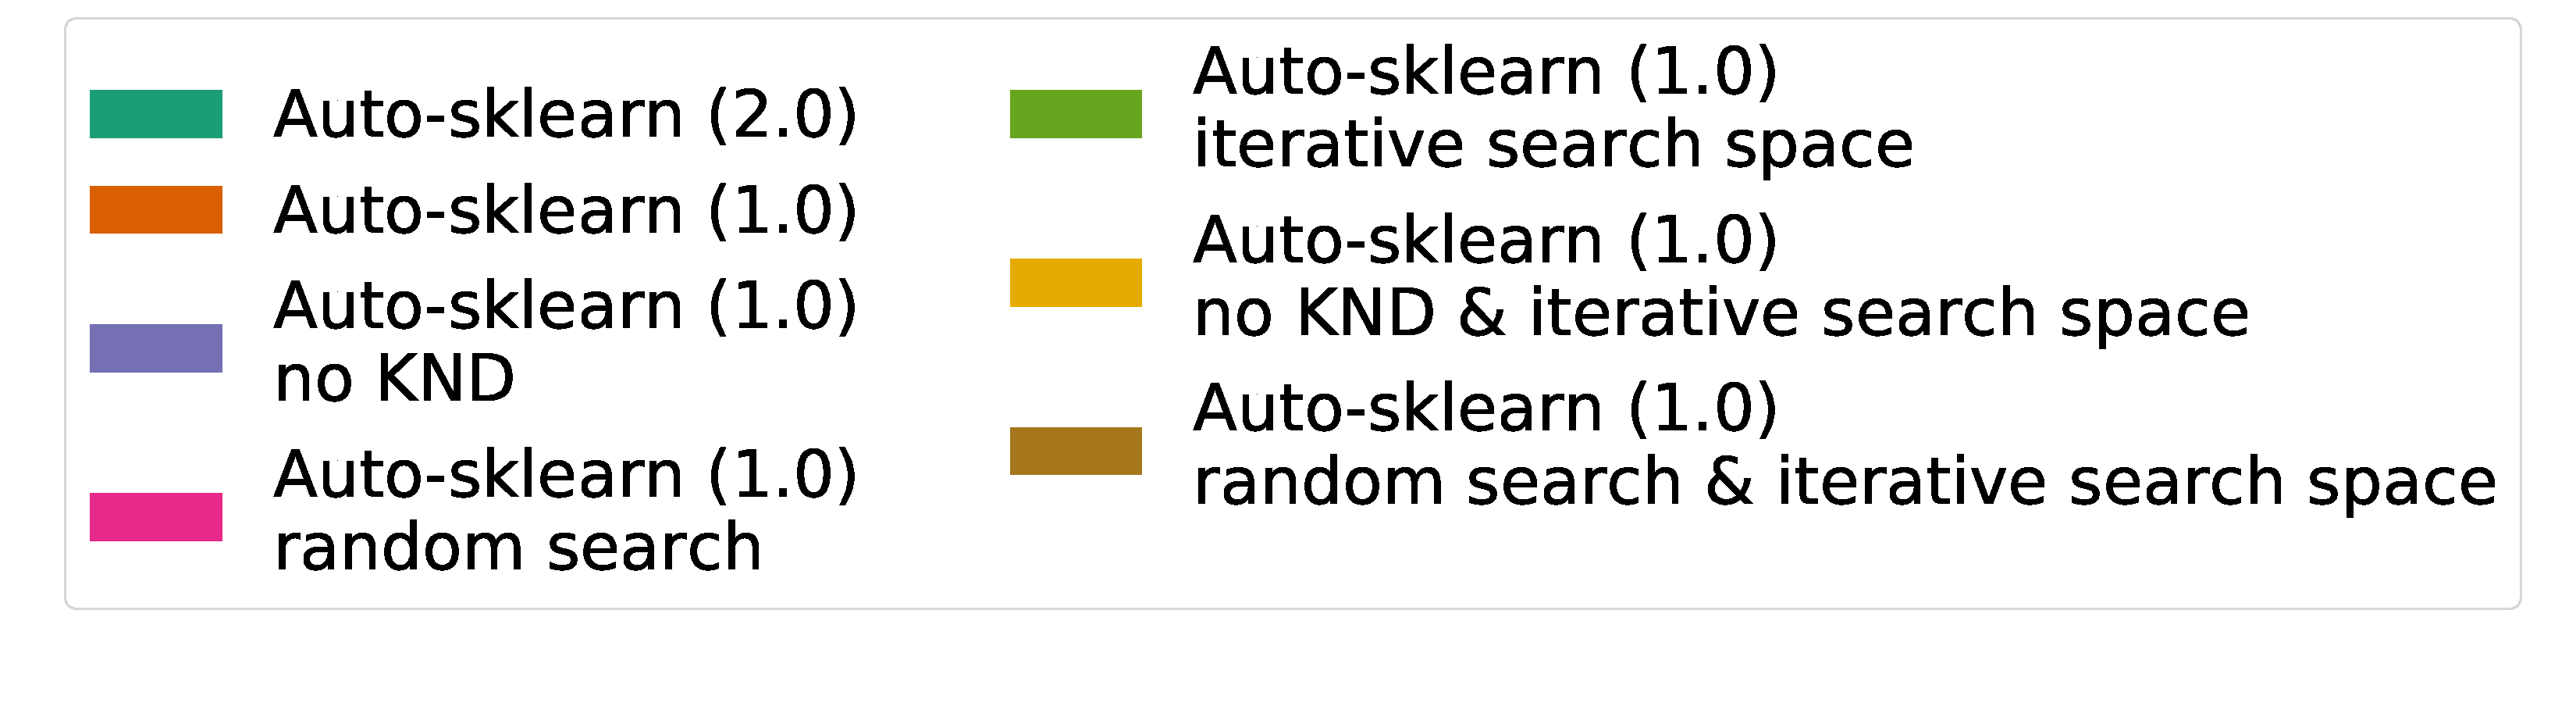
\includegraphics[width=\textwidth]{../w07_hpo_speedup/images/success_stories/RQ1_legend.pdf}
    \label{fig:my_label}
\end{figure}
\end{columns}

\end{frame}
%-----------------------------------------------------------------------